%%
%% Beginning of file 'sample.tex'
%%
%% Modified 2005 December 5
%%
%% This is a sample manuscript marked up using the
%% AASTeX v5.x LaTeX 2e macros.

%% The first piece of markup in an AASTeX v5.x document
%% is the \documentclass command. LaTeX will ignore
%% any data that comes before this command.

%% The command below calls the preprint style
%% which will produce a one-column, single-spaced document.
%% Examples of commands for other substyles follow. Use
%% whichever is most appropriate for your purposes.
%%
%%\documentclass[12pt,preprint]{aastex}

%% manuscript produces a one-column, double-spaced document:

%\documentclass{article}
%\documentclass[twocolumn]{aastex6}
\documentclass[iop]{emulateapj}

%% preprint2 produces a double-column, single-spaced document:
%\documentclass[preprint2]{aastex}

%% Sometimes a paper's abstract is too long to fit on the
%% title page in preprint2 mode. When that is the case,
%% use the longabstract style option.

%% \documentclass[preprint2,longabstract]{aastex}

%% If you want to create your own macros, you can do so
%% using \newcommand. Your macros should appear before
%% the \begin{document} command.
%%
%% If you are submitting to a journal that translates manuscripts
%% into SGML, you need to follow certain guidelines when preparing
%% your macros. See the AASTeX v5.x Author Guide
%% for information.

%Packages
\usepackage[colorlinks=true,linkcolor=blue,citecolor=blue]{hyperref}

\usepackage{natbib}
\bibliographystyle{astroads}

\newcommand{\vdag}{(v)^\dagger}
\newcommand{\DHSres}{272 - 304}

%% You can insert a short comment on the title page using the command below.

%\slugcomment{DHS White Paper}

%% If you wish, you may supply running head information, although
%% this information may be modified by the editorial offices.
%% The left head contains a list of authors,
%% usually a maximum of three (otherwise use et al.).  The right
%% head is a modified title of up to roughly 44 characters.
%% Running heads will not print in the manuscript style.

\shorttitle{JWST NIRCam SW and LW}
\shortauthors{Schlawin et al.}

%% This is the end of the preamble.  Indicate the beginning of the
%% paper itself with \begin{document}.

\begin{document}

%% LaTeX will automatically break titles if they run longer than
%% one line. However, you may use \\ to force a line break if
%% you desire.

\title{Two NIRCam Arms are Better than One: How JWST Can Do More Science with NIRCam's Short-Wavelength Dispersed Hartmann Sensor}

%% Use \author, \affil, and the \and command to format
%% author and affiliation information.
%% Note that \email has replaced the old \authoremail command
%% from AASTeX v4.0. You can use \email to mark an email address
%% anywhere in the paper, not just in the front matter.
%% As in the title, use \\ to force line breaks.

\author{E. Schlawin, M. Rieke, J. Leisenring, L. M. Walker, J. Fraine?, D. Kelly, K. Misselt}
\affil{Steward Observatory, Tucson AZ 85721}
\email{eas342@email.arizona.edu}

\author{T. Greene}
\affil{NASA Ames Research Center, Moffett Field, CA 94035}

\author{M. Line?\altaffilmark{1,2,3,4}}
\affil{Department of Astronomy and Astrophysics, University of California, Santa Cruz, CA 95064}

\author{N. Lewis?, J. Stansberry}
\affil{Space Telescope Science Institute, 3700 San Martin Drive, Baltimore, MD 21218, USA}

%% Notice that each of these authors has alternate affiliations, which
%% are identified by the \altaffilmark after each name.  Specify alternate
%% affiliation information with \altaffiltext, with one command per each
%% affiliation.

\altaffiltext{1}{Hubble Postdoctoral Fellow}
\altaffiltext{2}{NASA Ames Research Center, Moffett Field, CA 94035}
\altaffiltext{3}{Bay Area Environmental Research Institute, Petaluma, CA}
\altaffiltext{4}{School of Earth and Space Exploration, Arizona State University, Tempe, AZ}

%% Mark off your abstract in the ``abstract'' environment. In the manuscript
%% style, abstract will output a Received/Accepted line after the
%% title and affiliation information. No date will appear since the author
%% does not have this information. The dates will be filled in by the
%% editorial office after submission.

\begin{abstract}
James Webb Space Telescope (JWST) offers unprecedented sensitivity, stability and wavelength coverage for transiting exoplanet studies, opening up new avenues for measuring atmospheric abundances, structure and temperature profiles.
Taking full advantage of JWST spectroscopy of planets from 0.6 $\mu$m to 28$\mu$m, however, will require many observations with a combination of the NIRISS, NIRCam, NIRSpec and MIRI instruments.
In this white paper, we discuss a new NIRCam mode (not yet approved and implemented) that can reduce the number of observations needed for observations in the 1.0$\mu$m to 5.0$\mu$m wavelength range.
The NIRCam instrument was primarily designed as an imager, but includes several grisms for phasing and aligning JWST's 18 hexagonal mirror segments.
NIRCam's long-wavelength arm includes grisms that cover 2.4$\mu$m to 5.0$\mu$m with two observations at $R = 1200 - 1550$ and it has already been approved for wide field slitless spectroscopy.
We propose a new mode that will simultaneously measure spectra for science targets in the 1.0$\mu$m to 2.0$\mu$m range using NIRCam's short-wavelength arm.
This mode, if approved, would take advantage of NIRCam's Dispersed Hartmann Sensor (DHS), which produces 10 spatially separated spectra per source source at $R \sim \DHSres$.
The DHS can observe the brightest host stars of any JWST mode.
We discuss the added benefit of the DHS in constraining abundances in exoplanet atmospheres.
The DHS essentially comes for free with any NIRCam long-wavelength grism observation, but the readout has to be selected to ensure that the long-wavelength grism observations do not saturate and that the high frame rate images on 3 simultaneous detectors does not exceed the data volume JWST can downlink.
Combining both of NIRCam's arms will maximize the science potential of JWST, which is a limited life observatory.
\end{abstract}

%% Keywords should appear after the \end{abstract} command. The uncommented
%% example has been keyed in ApJ style. See the instructions to authors
%% for the journal to which you are submitting your paper to determine
%% what keyword punctuation is appropriate.

\keywords{telescopes, planets and satellites: atmospheres, instrumentation: spectrographs}

%% From the front matter, we move on to the body of the paper.
%% In the first two sections, notice the use of the natbib \citep
%% and \citet commands to identify citations.  The citations are
%% tied to the reference list via symbolic KEYs. The KEY corresponds
%% to the KEY in the \bibitem in the reference list below. We have
%% chosen the first three characters of the first author's name plus
%% the last two numeral of the year of publication as our KEY for
%% each reference.


%% Authors who wish to have the most important objects in their paper
%% linked in the electronic edition to a data center may do so by tagging
%% their objects with \objectname{} or \object{}.  Each macro takes the
%% object name as its required argument. The optional, square-bracket 
%% argument should be used in cases where the data center identification
%% differs from what is to be printed in the paper.  The text appearing 
%% in curly braces is what will appear in print in the published paper. 
%% If the object name is recognized by the data centers, it will be linked
%% in the electronic edition to the object data available at the data centers  
%%
%% Note that for sources with brackets in their names, e.g. [WEG2004] 14h-090,
%% the brackets must be escaped with backslashes when used in the first
%% square-bracket argument, for instance, \object[\[WEG2004\] 14h-090]{90}).
%%  Otherwise, LaTeX will issue an error. 

\section{Introduction}

The James Webb Space Telescope (JWST) \citep[e.g.][]{gardner2006SSRv} has the potential to profoundly expand and deepen the science of transiting exoplanets \citep[e.g.][]{greene2016jwst_trans}.
The wavelength coverage from 0.6$\mu$m to 28$\mu$m adds significantly to the wavelengths covered by the Hubble Space Telescope (HST) (currently 0.09$\mu$m to 1.7$\mu$m).
Its unprecedented infrared sensitivity and stable orbit at the second Lagrange (L2) point make it an excellent observatory for characterizing the atmospheres of planets that transit their host stars with time series observations.
Ground-based observatories and the Hubble Space Telescope have made important measurements of Na, K, H$_2$O in a variety of hot Jupiter, hot Neptune planets \cite[e.g.][]{snellen2008Na209,kreidberg2014wasp43,fraine2014hatp11,deming13,sing2016continuum}.
JWST has the capability of characterizing carbon-bearing molecules such as CH$_4$, CO and CO$_2$ to improve measurements of planet metallicity and C/O in comparison to it host star.
Depending on the composition and size of the clouds and hazes in exoplanet atmospheres, the longer wavelengths observed by JWST may penetrate these clouds and hazes.

No single JWST instrument may measure a spectrum over the full wavelength range from 0.6$\mu$m to 28$\mu$m, so multiple transits or secondary eclipses are necessary to piece together a broadband spectrum.
The largest bandwidths possible are NIRSpec's low resolution prism covering 0.7$\mu$m to 5$\mu$m and MIRI's low resolution prism (LRS) covering 5$\mu$m to 12$\mu$m.
Unfortunately, NIRSpec's low resolution prism mode is so sensitive, it saturates for most sources at a $J$ magnitude of $\sim$11 \citep{beichman2014pasp}, so many nearby bright planet systems must be observed with higher resolution (but smaller wavelength coverage) modes and instruments.
For example, to create a transmission spectrum for HD 209458b \citep{henry00,charbonneau00} from 0.7 $\mu$m to 12 $\mu$m, an observer would have to stitch together at least four different transits: one with NIRISS (0.7 to 2.5$\mu$m), two with NIRCam's long-wavelength arm (2.44$\mu$m to 4.98 $\mu$m) \footnote{Or, alternatively NIRSpec's G235H and G395H  grisms covering 1.7$\mu$ to 5.0$\mu$m.} and one with MIRI (5$\mu$m to 12$\mu$m).
With typical overheads of $\sim$2 hr for 9 hours of pre-ingress, transit and post-ingress, this totals to about ~11 hours per transit or 44 JWST hours.
This was calculated with the Astronomer's Proposal Tools software\footnote{http://www.stsci.edu/hst/proposing/apt} with the NIRISS SOSS mode, NIRCam's F322W2 and F444W grism time series and the MIRI Low Resolution spectrograph (LRS).

The NIRCam instrument is primarily an imager, but it includes several spectroscopic modes originally designed for wavefront sensing.
These include the grisms installed in its long-wavelength arm as well as the Dispersed Hartmann Sensors (DHSs) installed in its short-wavelength arm.
The long-wavelength grisms are used in concert with broadband filters.
The F322W2 filter encompasses 2.44$\mu$m to 4.02$\mu$m half maximum throughput while the F444W filter encompasses 3.88$\mu$ to 4.98$\mu$m at half maximum throughput.
These filters and grism are enabled and supported JWST science modes.
The DHS would be used primarily with the F150W2 filter, which covers from 1.01$\mu$m to 2.35$\mu$m at half maximum throughput.
The range from 2.0$\mu$m to 2.35$\mu$m will probably be discarded because the first order of the spectrum begins to overlap at at 2.0$\mu$m.

The NIRCam instrument can reduce the number of transits needed to build up a transmission or emission spectrum of a planet from 1$\mu$m to 5 $\mu$m.
This is because the instrument has a dichroic that splits the incoming beam into a short-wavelength arm and long-wavelength arm, so simultaneous imaging and/or spectroscopy are possible at short ($<$2.4$\mu$m) and long ($>$2.4$\mu$m) wavelengths.
In particular, the DHS can be used to simultaneously cover 1.0$\mu$m to 2.0$\mu$m while the long-wavelength grisms cover either 2.44$\mu$m to 4.02$\mu$m (with the F322W2 filter) or 3.88$\mu$m to 4.98$\mu$m (with the F444W) filter.
Thus, the DHS data comes ``for free'' with any long-wavelength NIRCam grism data, aside from readout and data rate considerations discussed in Section \ref{sec:readout}.
For the example above of HD 209458b, this could save about 11 JWST hours per transit if the wavelengths from 2.0 to 2.4$\mu$m and higher Signal to Noise ratios (SNRs) from NIRISS are not required.
The DHS is expected to perform similarly to HST's WFC3 grisms, so it is like a free coordinated HST observation for every long-wavelength NIRCam grism transit.

\begin{figure}[!ht]
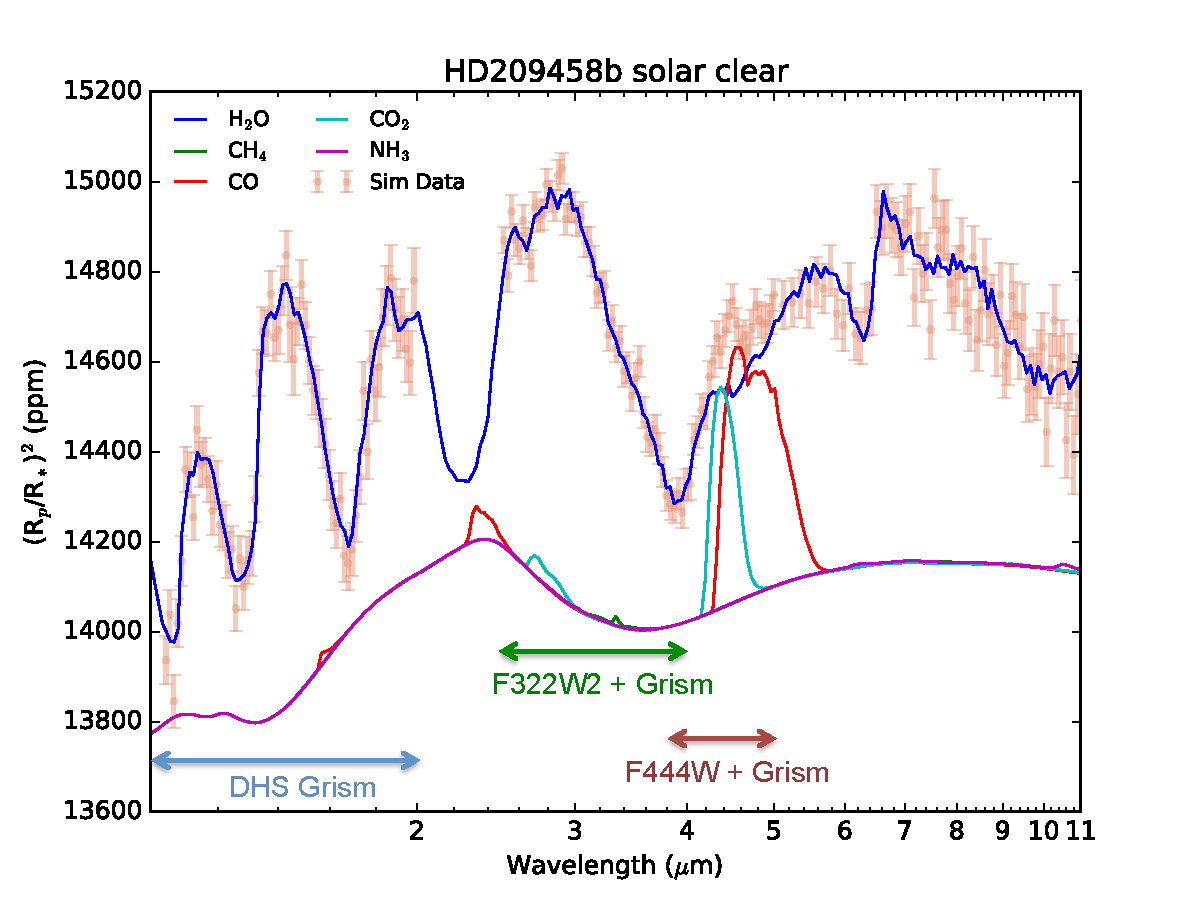
\includegraphics[width=0.5\textwidth]{molecules_DHS_HD209.pdf}
\caption{Model spectra separated by molecule for HD 209458b.
The new DHS mode would allow simultaneous spectra at 1-2$\mu$m ``for free'' when observing with either NIRCam's F322W2 or F444W slitless grism observations in its long-wavelength arm.
The simulated data are for one transit in each of the long-wavelength grism modes, each accompanied by simultaneous DHS grism spectra.
The observations longer than 5$\mu$m are simulated for MIRI's Low Resolution Spectrometer.}\label{fig:DHSmolecules}
\end{figure}

Since the DHS was not originally designed for science observations, it is not yet an approved mode for the James Webb Space Telescope.
In this white paper, we argue for the inclusion of the DHS mode to fully take advantage of two NIRCam arms to maximize JWST's science potential for transiting planets.
In section \ref{sec:addedScience} we discuss the added science that can be achieved with the DHS, including the brightness limits and improved precision in retrieved parameters for a representative system.
In section \ref{sec:implementation}, we discuss how the DHS would work for time-series observations and the implications of reading out several detectors simultaneously at a high frame rate.


\section{Science Benefits with the DHS}\label{sec:addedScience}

\subsection{Brightness limits}\label{sec:brightness}

The DHS has the best brightness limits of any spectroscopic mode on JWST because it spreads light over many pixels and reduces the effective aperture of JWST.
Figure \ref{fig:DHSaps} shows the saturation limits for the DHS mode along with NIRCam's long-wavelength grisms.
Any known transiting planet host system can be observed with the DHS, including the transiting super-Earth  55 Cnc e \citep{mcarthur2004disc55cnce} at $K$=4.0, which is right at the limit of saturation of the long-wavelength grism and the brightest known transiting system HD 219134b \citep{motalebi2015hd219134b} at $K$=3.4.
The DHS also enables characterization of any future targets found in this brightness range, such as by the Transiting Exoplanet Survey Satellite (TESS).

\begin{figure}[!ht]
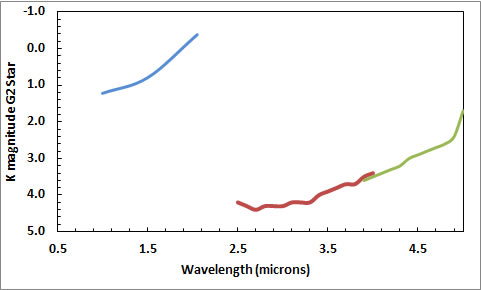
\includegraphics[width=0.5\textwidth]{sat_limits.jpg}
\caption{Saturation limits of the DHS mode (blue), and long-wavelength grism's F322W2 filter (red) and F444W filter (light green) for a G2V star.
The magnitudes are Vega K magnitudes where 80\% of the well depth is filled in the standard CDS readout mode described in Figure \ref{fig:readout}  for a 2048 $\times$ 64 pixel sub-array using 4 amplifiers.
The filters used are F150W2 (blue), F322W2 (red) and F444W (green).}\label{fig:DHSaps}
\end{figure}

\subsection{CHIMERA Simulations}\label{sec:simulations}

We use the CHIMERA atmospheric retrieval suite \citep{line2013chimera,line2014CtOsecE} to show the scientific value of using the DHS simultaneously with NIRCam's long-wavelength grisms.
We first simulate a forward model of a transmission spectrum for a planet (in this case HD 209458b).
We then add Gaussian noise using the SNR estimated on the target to create a simulated spectrum.
Finally, we run a Markov Chain Monte Carlo (MCMC) retrieval of the atmospheric parameters for simulated spectrum to try to recover the initial abundances and determine the uncertainties in those abundances, as in \citet{greene2016jwst_trans}.
We combine the individual gases' posterior distributions for the C/O ratio and metallicity.

\begin{figure}
\centering
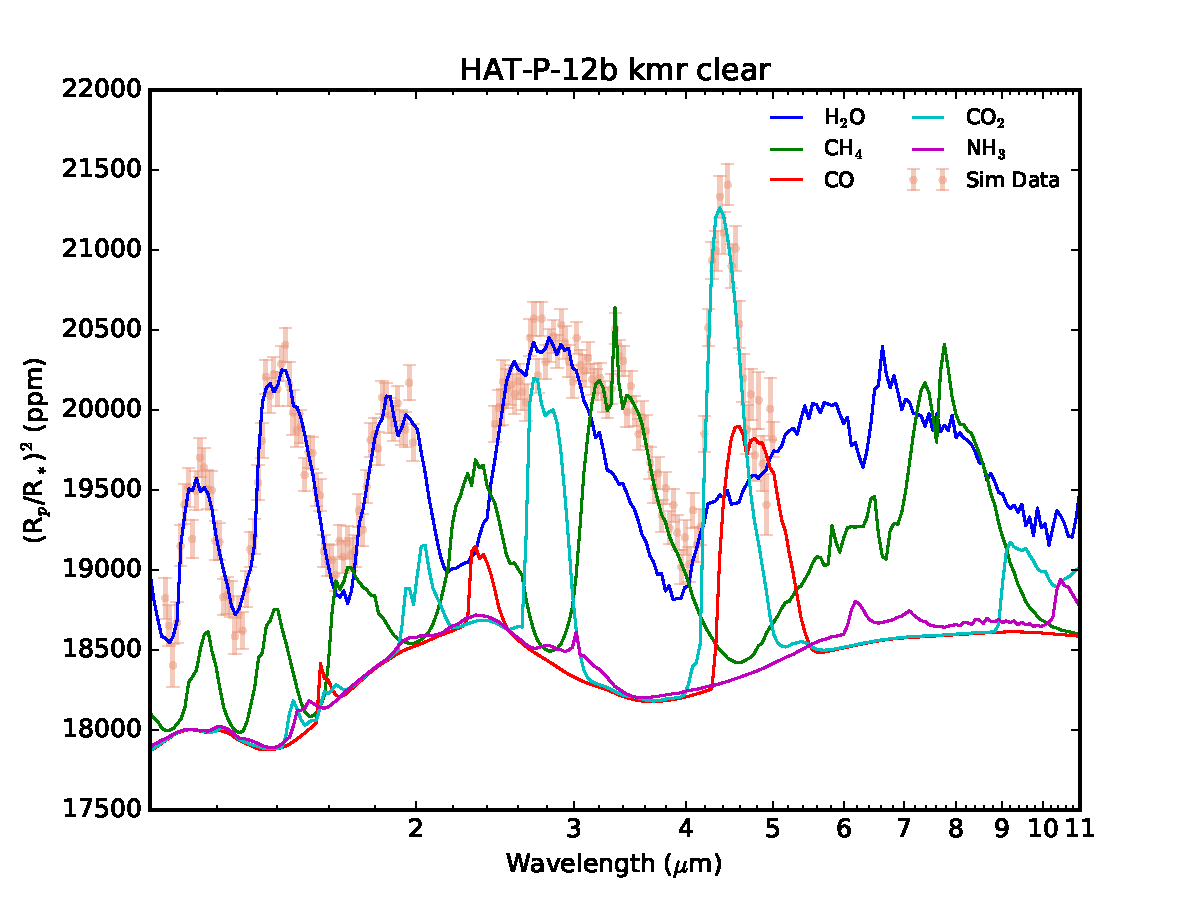
\includegraphics[width=0.5\textwidth]{HAT-P-12b_kmr_clear_DHS_nc.pdf}
\caption{Model spectra separated by molecule for for the inflated warm Saturn HAT-P-12b.
Error bars shown are for simulated observation with the DHS grism, F322W2 and F444W modes, for a total of 2 transits or about 17 hours of JWST time.}\label{fig:DHSvsNIRISS209}
\end{figure}

For the initial model, we use solar abundances of \citet{asplund} and reduce the oxygen by a factor of 24\% to account for the settling out of MgSiO$_3$ and MgSiO$_4$ which are below their condensation temperatures \citep{sing2016continuum}.
The atomic abundances are converted to molecular mixing ratios using the Chemical Equilibrium code with Applications (CEA) \footnote{http://www.grc.nasa.gov/WWW/CEAWeb/ceaHome.htm}\citep{gordon1996cea} to calculate the fractions of molecules at the given pressure and temperature.
For HD209458b, this is at a reference pressure of 0.01 bars and a reference temperature of 1440K.
We assume that the abundances and temperature are constant with altitude.
We include H$_2$O, CO, CO$_2$, CH$_4$, NH$_3$, C$_2$,H$_2$, HCN and collision-induced absorption (CIA) of hydrogen as sources of opacity, but only H$_2$O, CO, and CO$_2$ contribute significantly to the opacity, as seen in Figure \ref{fig:DHSmolecules}.
% if we run the simulations later, also mention emission spectra

For the simulated observations, we assume one transit is obtained in each of NIRCam's long-wavelength filters (F322W2 and F444W) to cover the wavelength range from 2.44$\mu$m to 4.99$\mu$m.
We assume that each of these was accompanied by a DHS observation for the 1.01$\mu$m to 2.0$\mu$m wavelength range, which benefits in SNR by $\sqrt(2)$ for the two separate observations.
This is compared to observations taken without the DHS to show the added scientific value of using the DHS spectra.
The noise models for the hot Jupiter HD 209458b are shown in Figure \ref{fig:DHSvsNIRISS209}, which is dominated by the detector noise floor (35 ppm) for the long-wavelength grisms ($>$2.44$\mu$m) but photon noise is more significant for the short-wavelength DHS observations.
The DHS has lower throughput and a smaller wavelength coverage than the NIRISS instrument in SOSS mode, so observations which require higher SNR and full wavelength coverage from 0.7 to 2.4$\mu$m can take advantage of NIRISS (also shown in Figure \ref{fig:DHSvsNIRISS209}) at the expense of more telescope time.

\begin{figure}
\centering
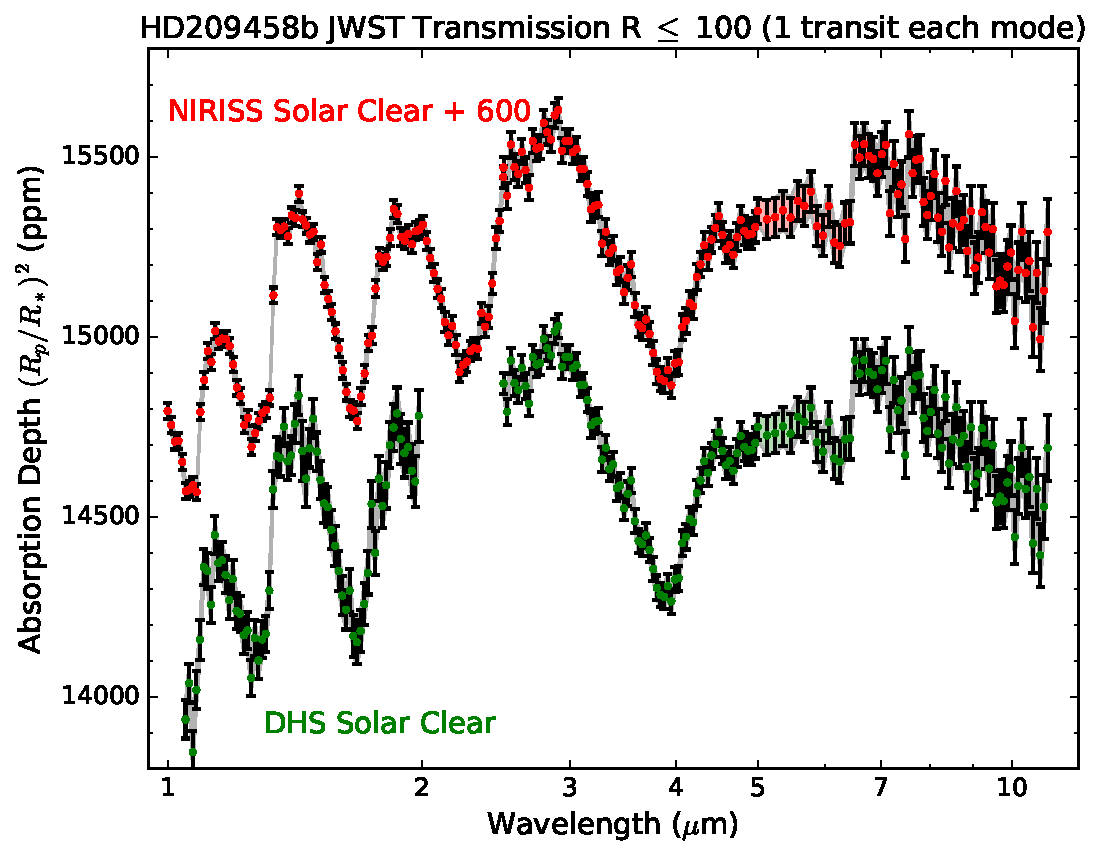
\includegraphics[width=0.5\textwidth]{HD209458b_solar_clear_1transit_DHS_vs_NIRISS_NIRCam_MIRILRS_R100.pdf}
\caption{Calculated SNR for one transit of the hot Jupiter HD209458b for the NIRISS SOSS mode, NIRCam F322W2 and F444W filters and the MIRI LRS mode for a total of 4 different transits or $\sim$44 JWST hours.
Similar wavelength coverage can be achieved in just 3 different transits or $\sim$ 33 hours if the DHS mode is enabled (bottom spectrum).}\label{fig:DHSvsNIRISS209}
\end{figure}

We use CHIMERA and a Markov Chain Monte Carlo (MCMC) retrieval to recover the individual atmospheric abundances of the simulated spectrum.
The retrieval model includes 13 free parameters: 1) the temperature of the isothermal profile 2) the altitude of the 10-bar pressure surface where the model begins 3) a cloud pressure level below which all stellar flux is absorbed at all wavelengths 4-11) the abundances of H$_2$O, CH$_4$, CO, CO$_2$, NH$_3$, C$_2$H$_2$, HCN, N$_2$, respectively 12) an amplitude of a Raleigh-like haze and 13) a power law index for the Raleigh-type haze.
We assume flat priors in log space for all abundances from volume mixing ratios of 10$^{-12}$ to 1.
The autocorrelation time for the retrievals is about ~100 steps and we run all retrievals to 20,000 steps, only using the last 5,000 to allow for burn-in.

%\begin{figure}
%\centering
%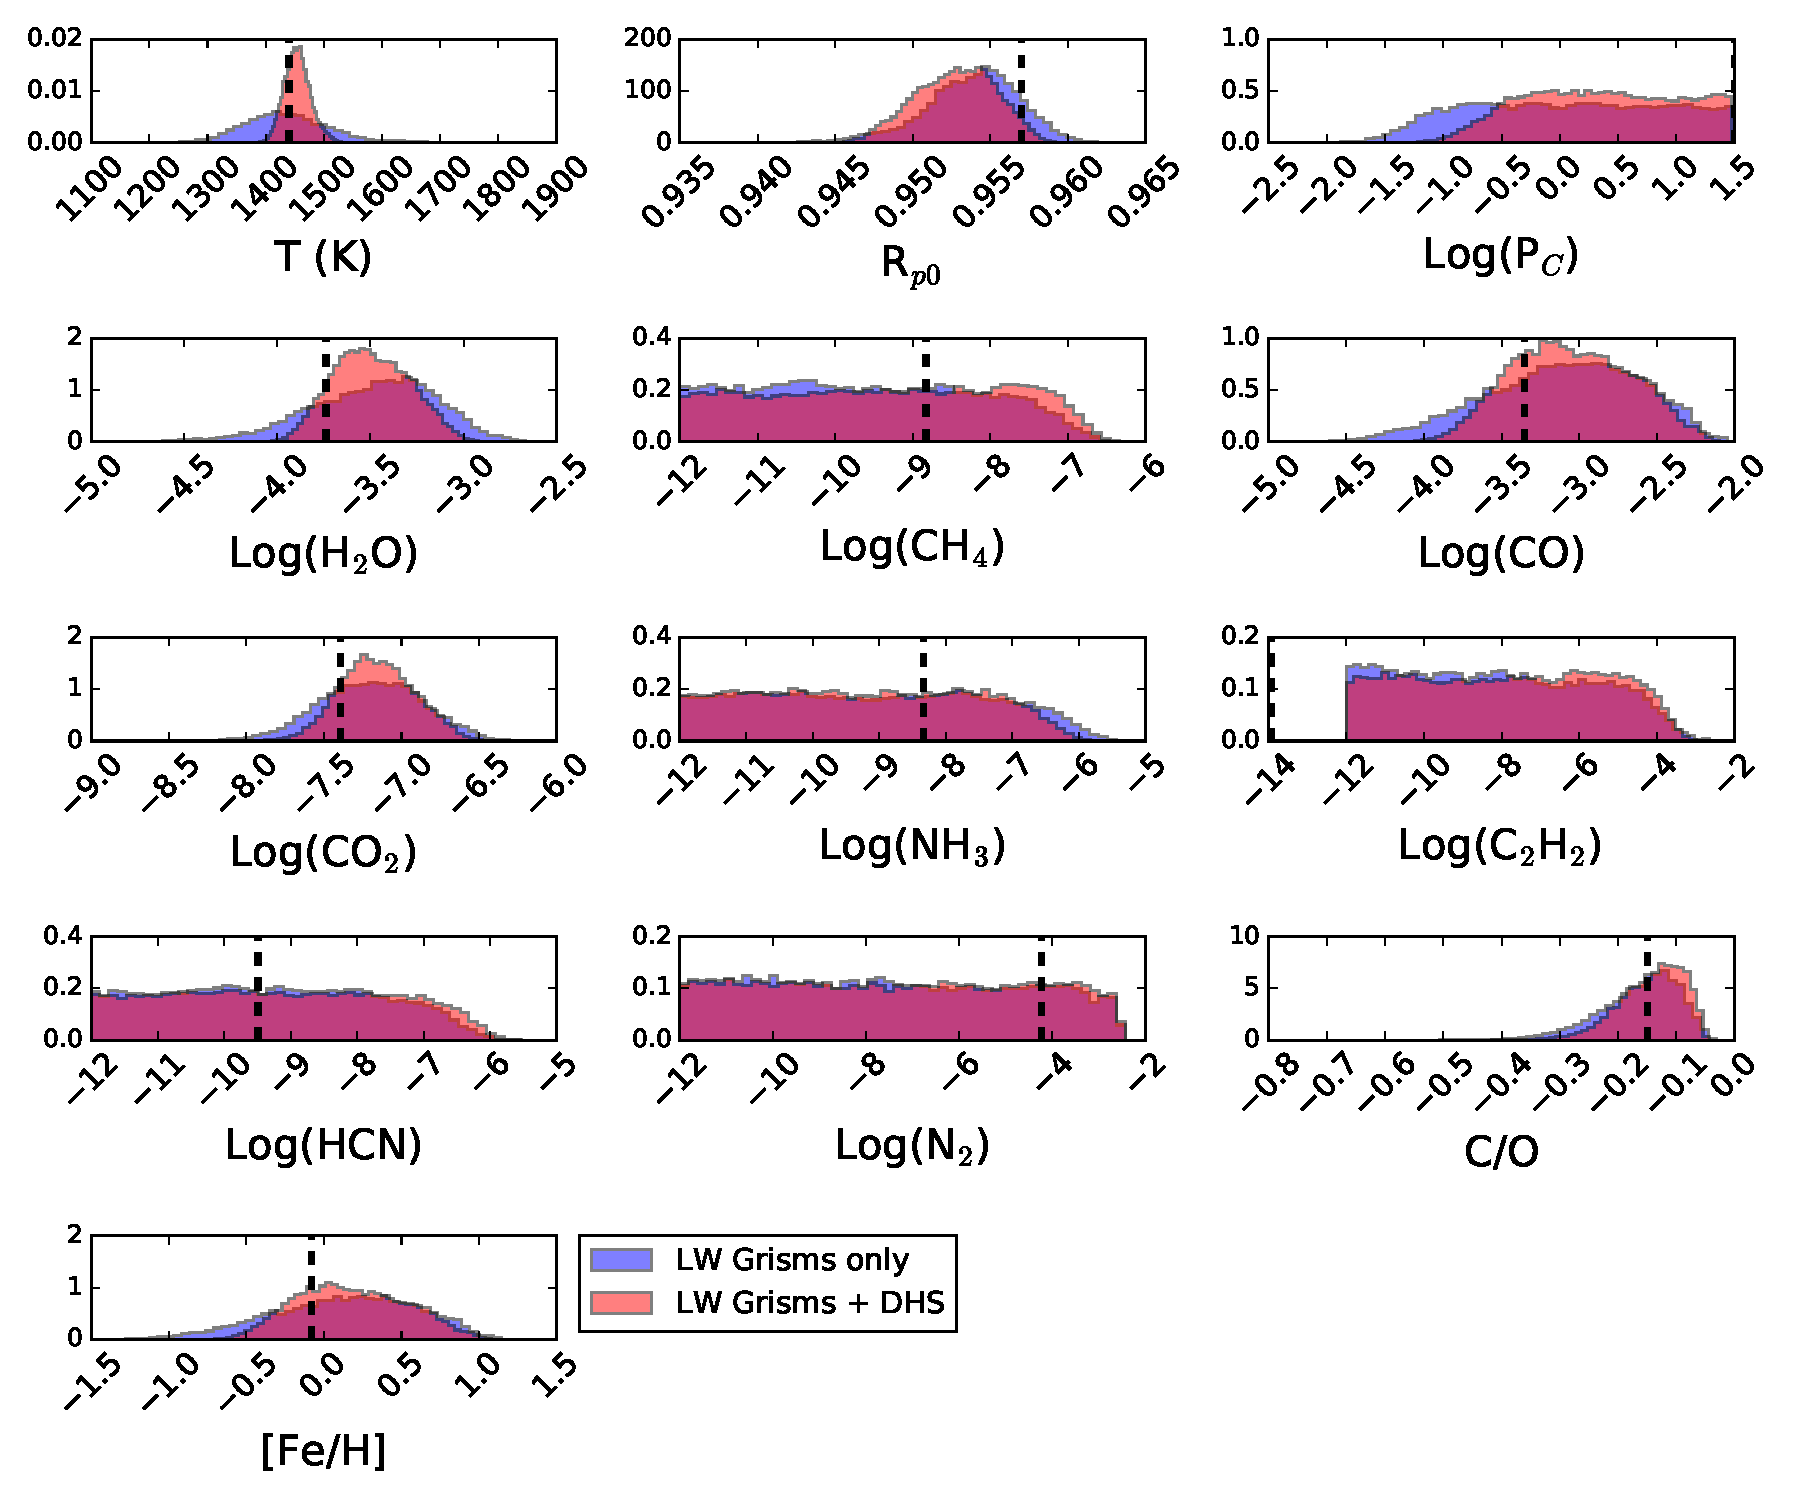
\includegraphics[width=0.5\textwidth]{HD209458b_solar_clear_DHS.pdf}
%\caption{Posterior distributions of the retrieved abundances, showing improvements of the constraints on temperature, cloud pressure upper limit and H$_2$O, CO$_2$ and CO abundances with the DHS.
%Vertical dashed bars show the input abundances for the initial forward model that was used to generate the simulated spectru.}\label{fig:DHSposterios}
%\end{figure}

\begin{figure*}
\centering
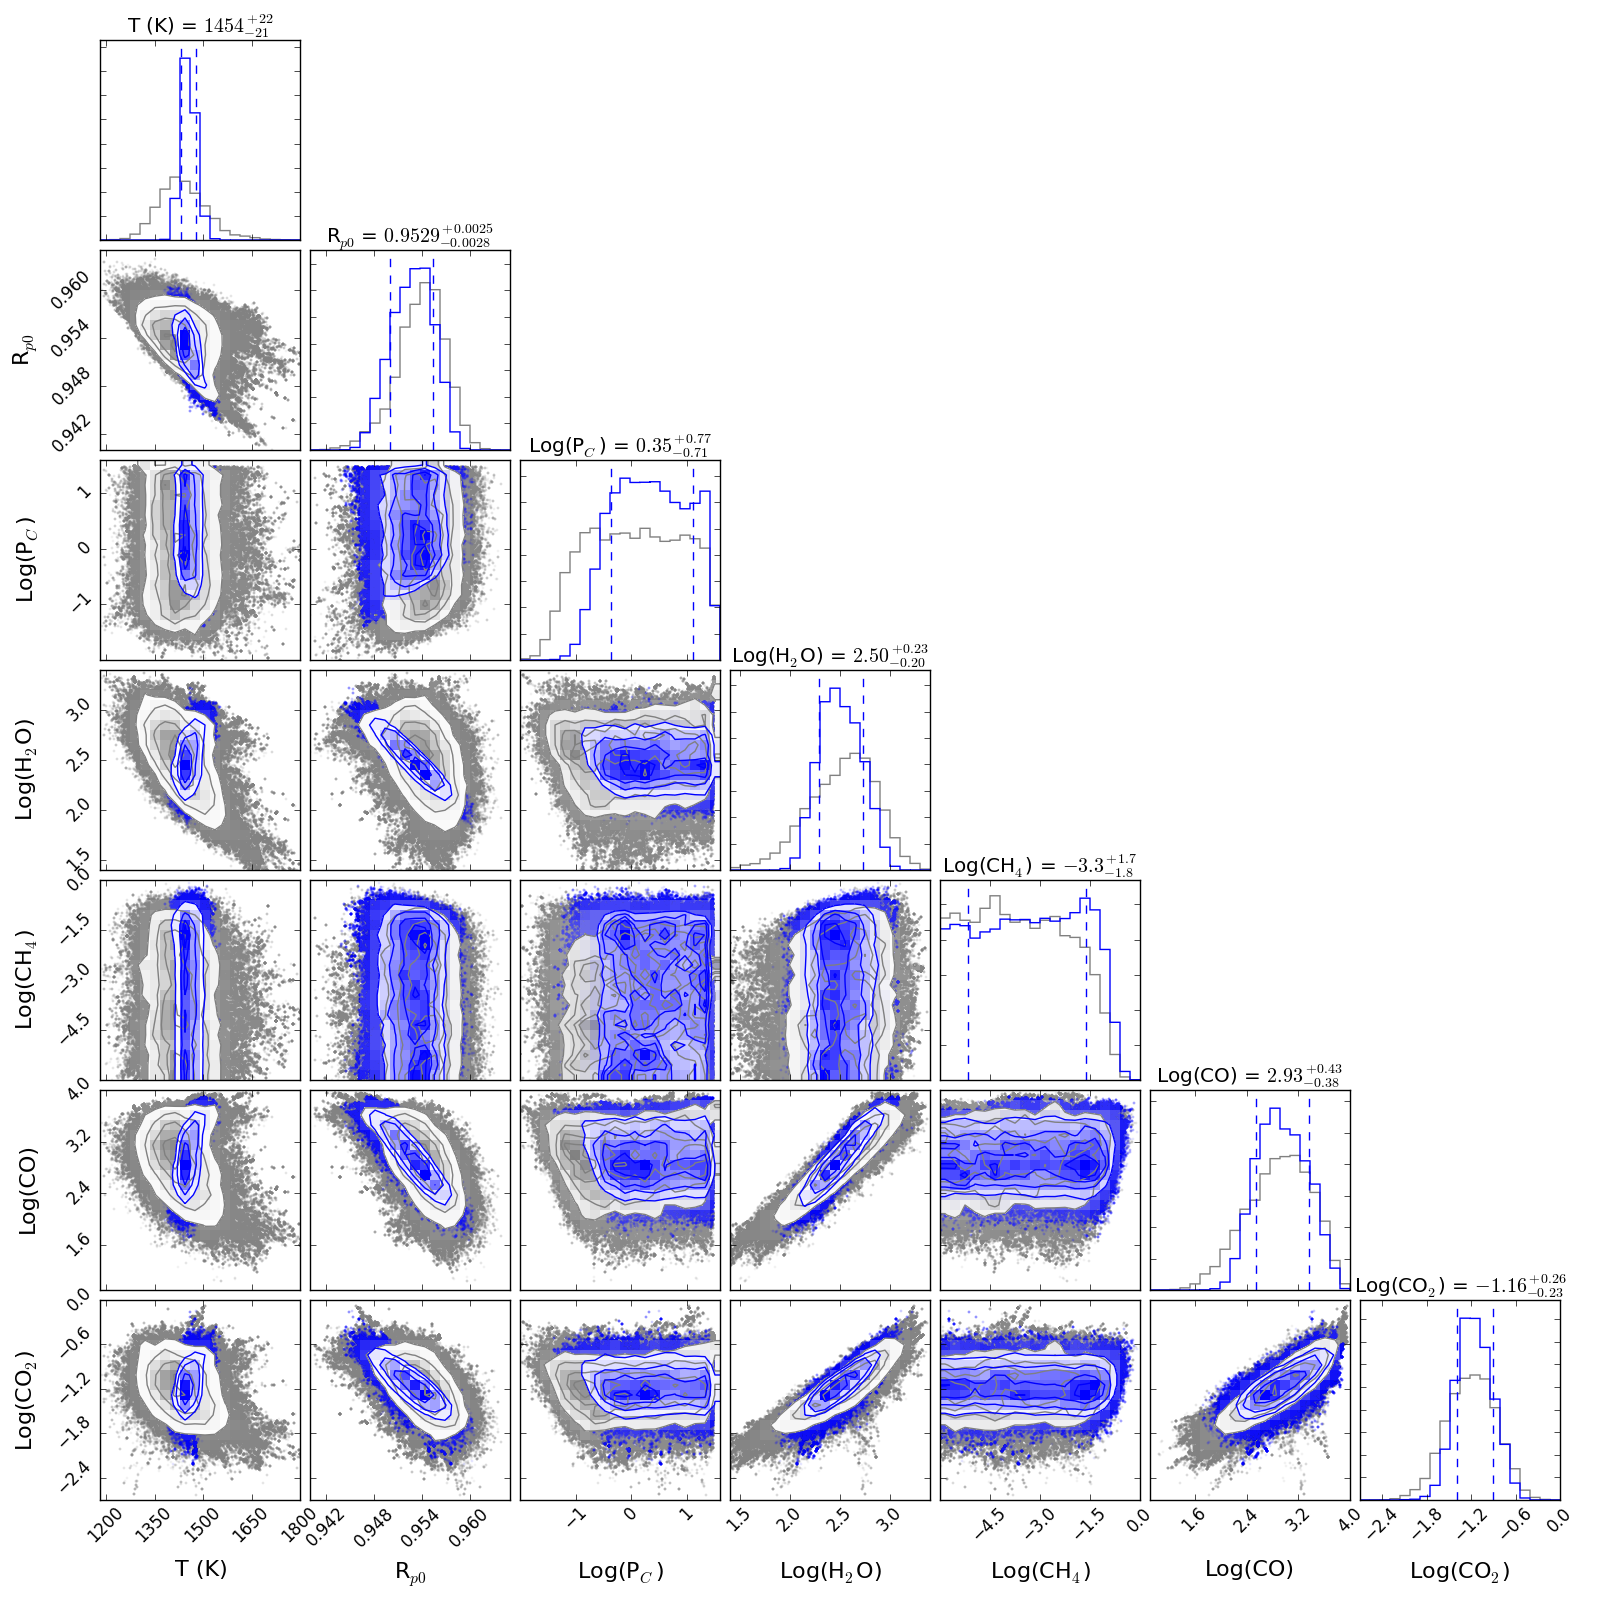
\includegraphics[width=1.0\textwidth]{HD209458b_solar_clear_1trans_corner.png}
\caption{Posterior distributions an MCMC run of HD209458b with the DHS (blue) and without the DHS (gray).
The H$_2$O correlates strongly with CO$_2$ and CO, meaning that improved measurements of H$_2$O with the DHS actually help improve constraints on the Carbon bearing species, even though there aren't any significant CO or CO$_2$ features in the 1-2$\mu$m range.}\label{fig:cornerRun}
\end{figure*}

One of the surprising aspects to the retrievals is that the DHS improves both the constraints on the CO and CO$_2$ abundances as well as the H$_2$O abundances, seen in Figure \ref{fig:cornerRun}.
A quick glance at the contributions of individual molecules to the spectrum shown in Figure \ref{fig:DHSmolecules} would indicate that the DHS is mainly important for water vapor.
However, the retrieval for the spectrum with only NIRCam's long-wavelength grisms has a strong correlation between the retrieved H$_2$O abundances with CO$_2$ and CO, shown in Figure \ref{fig:cornerRun}.
Improving the water vapor constraint with the DHS, reduces the correlation and therefore improves the abundance constraints for all three.

\section{DHS Implementation}\label{sec:implementation}

\subsection{DHS properties}
The DHS expands the wavelength range that NIRCam can achieve on a single observation by simultaneously obtaining spectroscopy with NIRCam's short wavelength arm and long wavelength arm.
The wavelength range for the F150W2 filter in the short wavelength arm is fixed at 1.01 to 2.02$\mu$m with the region from 2.02-2.35$\mu$m contaminated by second order overlap.
The DHS are slitless, so the resolution is set by the pupil sizes of the individual DHS elements, which are approximately the same width in the dispersion direction.
Figure \ref{fig:DHSRes} shows the resolution as a function of wavelength, estimated from the spatial PSF and the aspect ratio of dispersion and spatial directions.
There will be about a 0.04$\mu$m gap in the spectrum due to the gap between short wavelength detectors.
The center of this gap depends on source position.
The DHS can be used in tandem with either the F322W2 or F444W filter for the long wavelength grism observations.
The The properties of the DHS, which can be used simultaneously with the long-wavelength grisms, are listed in Table \ref{tab:DHSgprop}.
If the region from 2-2.2 is highly desirable, the DHS can be used with a F200W filter (1.75 to 2.23$\mu$m half maximum) to partially fill in the gap between the short to long wavelength arms.

\begin{figure}[!ht]
\centering
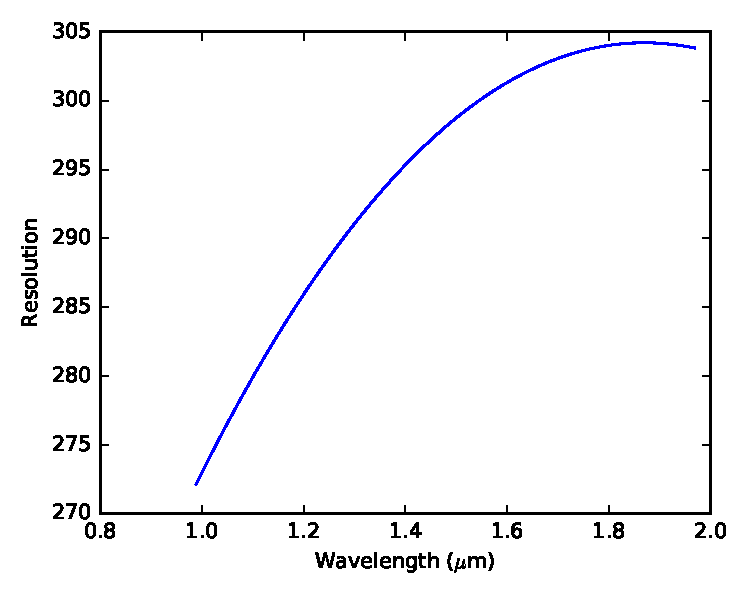
\includegraphics[width=0.4\textwidth]{dhs_res.pdf}
\caption{Resolution as a function of wavelength for the DHS.}\label{fig:DHSRes}
\end{figure}

\begin{table}
\centering
\begin{tabular}{ccr}
		& DHS	& Grism \\
 \hline \hline		
Resolution &  \DHSres & 1200 - 1550 \\
Dispersion & 0.29 nm / px & 1.0 nm / px \\
Wavelengths & 1.01 - 2.02$\mu$m (F150W2)\footnote{There is a 0.05$\mu$m gap between detectors that depends on field position} & 2.44 - 4.02$\mu$m (F322W2)\\
				& 								& 3.88 - 4.98$\mu$m (F444W) \\
Plate Scale & 32 mas/px  &  65 mas / px\\
\hline
\end{tabular}
\caption{Properties of DHS and simultaneous long-wavelength grism spectra.}\label{tab:DHSgprop}
\vspace{0.1in}
\end{table}

\subsection{DHS Layout}

A point source observed with the DHS and grism modes of NIRCam will produce 10 spectra on the short-wavelength arm and one spectrum on the long-wavelength arm -- see Figure \ref{fig:DHSimage}.
The DHS spectra span two of NIRCam's short-wavelength detectors covering 1-2$\mu$m with a 0.05$\mu$m due to the separation between detectors.
The DHS mode is well suited for one bright source because it spreads the light over the 10 separate spectra, but would be ill-suited for a crowded field, where the spectra would overlap.
Each of the DHS spectra are separated in the spatial direction by an average of 123 pixels, so a sub-array of at least 1300 pixels must be extracted to gather all DHS flux for a single source.
Each DHS spectrum roughly covers 4\% of the JWST pupil, though they vary in size and throughput depending on where they lie relative to the secondary mirror strut supports, seen in Figure \ref{fig:DHSvsPupilOverlay}.
We elected to clock the pupil wheel by 1.9$^\circ$ in order to align the spectra with rows on the short wavelength detector.
Aligning spectra along the rows enables small stripe mode readouts (such as 2048 $\times$ 64) to read one DHS spectra simultaneously with long wavelength grism spectra.
This is needed for bright targets that will saturate the long wavelength detector with longer frame times, as shown in Section \ref{sec:readout}.
There is a price for clocking the DHS pupil wheel to align spectra with rows: all DHS grisms are partially obscured, save element 7.
Fortunately, the relative obscuration for all 10 DHS spectra is small, going from 32\% when the pupil wheel is centered (which produces tilted spectra), versus 29\% if the pupil wheel is clocked to align the spectra along rows.
Table \ref{tab:pupfrac} lists the fractional pupil coverage of each DHS spectrum where 1.00 would use the entire pupil and JWST collecting area.
For a sub-array size encompassing only 1 DHS spectrum (such as a 2048 $\times$ 64 subarray), the largest unobscured DHS grisms should be used - element number 7 in Figure \ref{fig:DHSvsPupilOverlay}.

%The two DHS pupil configurations include 10 prisms spanning adjoining edges of JWST's hexagonal mirrors, at 60 degrees from each other to encompass different mirror pairs.
%The resulting image, shown in Figure \ref{fig:DHSimage} is that 10 separate spectra are produced for every point source covering the wavelengths from 1$\mu$m to 2$\mu$m.
%If two JWST mirrors are misaligned, they will produce a ``barber pole''-shaped interference pattern on the array.
\begin{figure}[!ht]
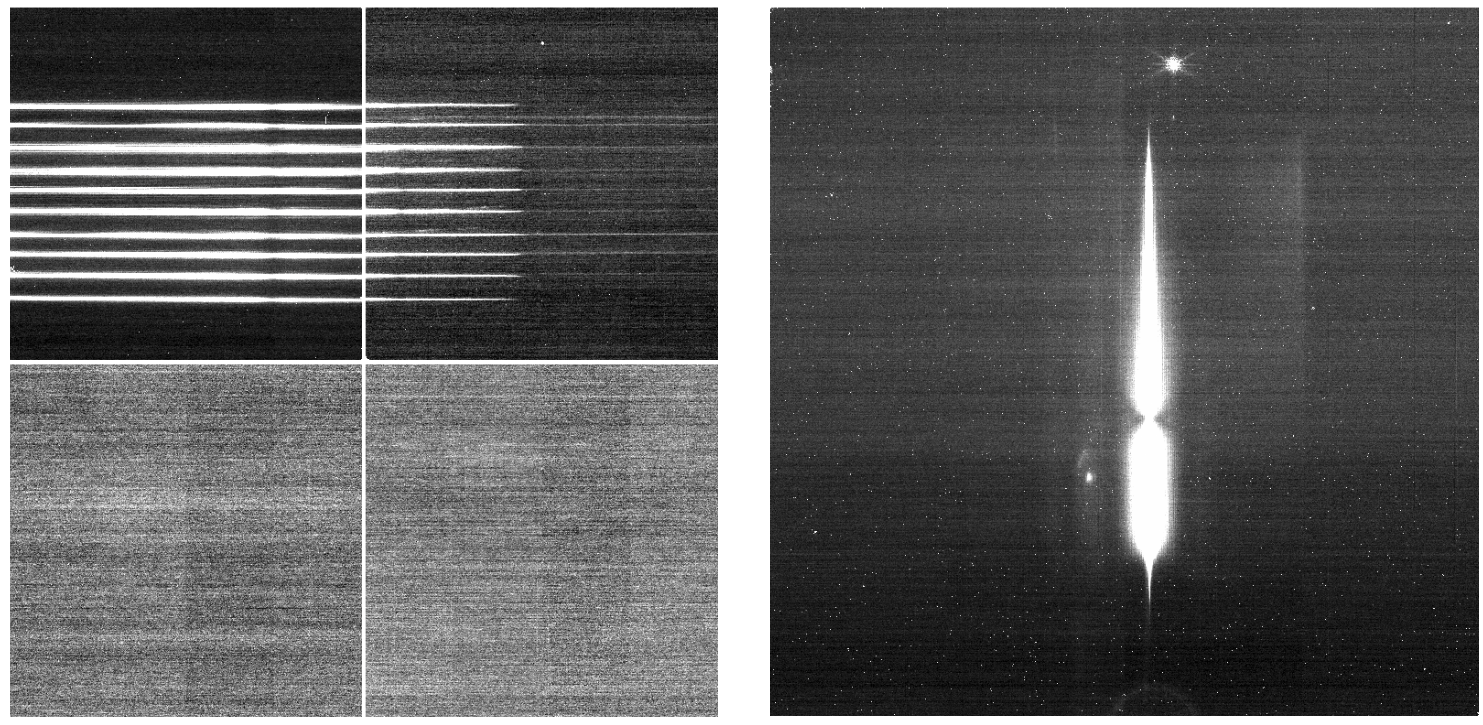
\includegraphics[width=0.5\textwidth]{dhs_image_example.png}
\caption{Example images of the same source observed simultaneously with the DHS on the short-wavelength arm (left) producing 10 spectra and the F444W filter and C grism on the long-wavelength arm (right).
These images were taken during cryogenic vacuum testing of the NIRCam flight instrument and detectors at NASA Goddard.
Only 3 detectors will be needed for transit observations \textbf{Update w/ Mod A image and w/ R grism estimate}.}\label{fig:DHSimage}
\end{figure}

\begin{table}
\centering
\begin{tabular}{cc}
DHS \# & Pupil Fraction \\
\hline \hline
1 & 0.012 \\
2 & 0.032 \\
3 &  0.032 \\
4 & 0.040 \\
5 & 0.021 \\
6 & 0.015 \\
7 & 0.042 \\
8 & 0.040 \\
9 & 0.036 \\
10 & 0.022 \\
\hline
Total & 0.292
\end{tabular}
\caption{Pupil Coverage}\label{tab:pupfrac}
\tablecomments{The approximate pupil coverage of the 10 DHS grisms compared to the total primary collecting area.}
\end{table}

\begin{figure}
\centering
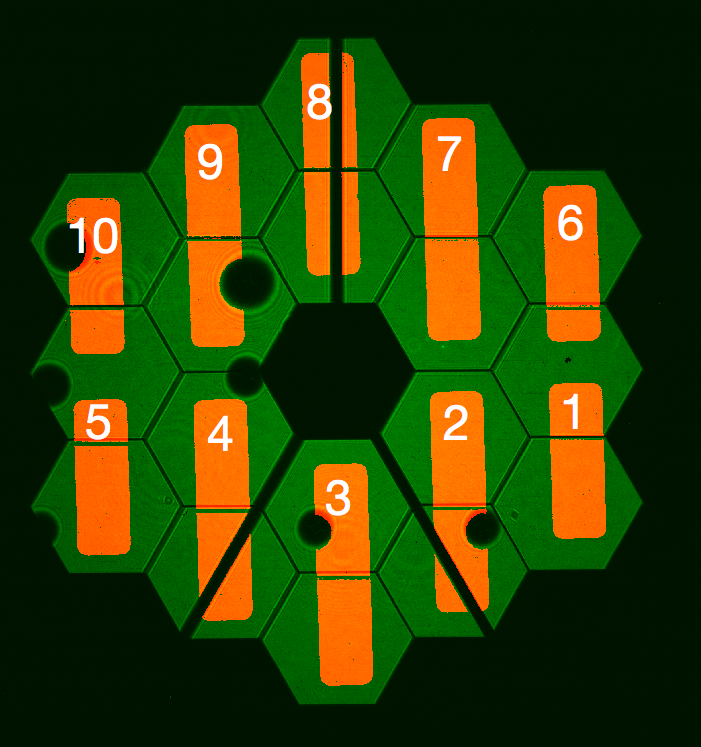
\includegraphics[width=0.4\textwidth]{dhs_pupil_overlay.png}
\caption{DHS pupil coverage by each of the 10 DHS prisms, with the fractional throughput given in Table \ref{tab:pupfrac}. 
The throughput is modulated by the size of the DHS grism as well as whether it coincides with a secondary mirror support (black lines).
The circles in the image are products of the OSIM (optical telescope element simulator) test source used in Cryogenic Vacuum testing of the instrument suite, and will not be present in flight.
The pupil wheel is clocked to make the DHS spectra straight along rows, but this moves the DHS elements off-center from JWST's pupil and masks.
\textbf{Remove circles and secondary struts from Orange}}\label{fig:DHSvsPupilOverlay}
\end{figure}

\subsection{Readout Considerations}\label{sec:readout}
JWST's NIRCam has many different possible readout patterns per pixel and array that all factor in to the SNRs and saturation limits for an observation.
We adopt the following naming convention for the readout: An observation may consist of one of more exposures which are typically combined into a single \texttt{FITS} file per exposure.
Within an exposure, there are 1 or more integrations, which consist of a reset frame followed by 1 or more groups of non-destructive reads up a ramp.
This is illustrated in Fig \ref{fig:readout} for three example readout modes.

\begin{figure}
\centering
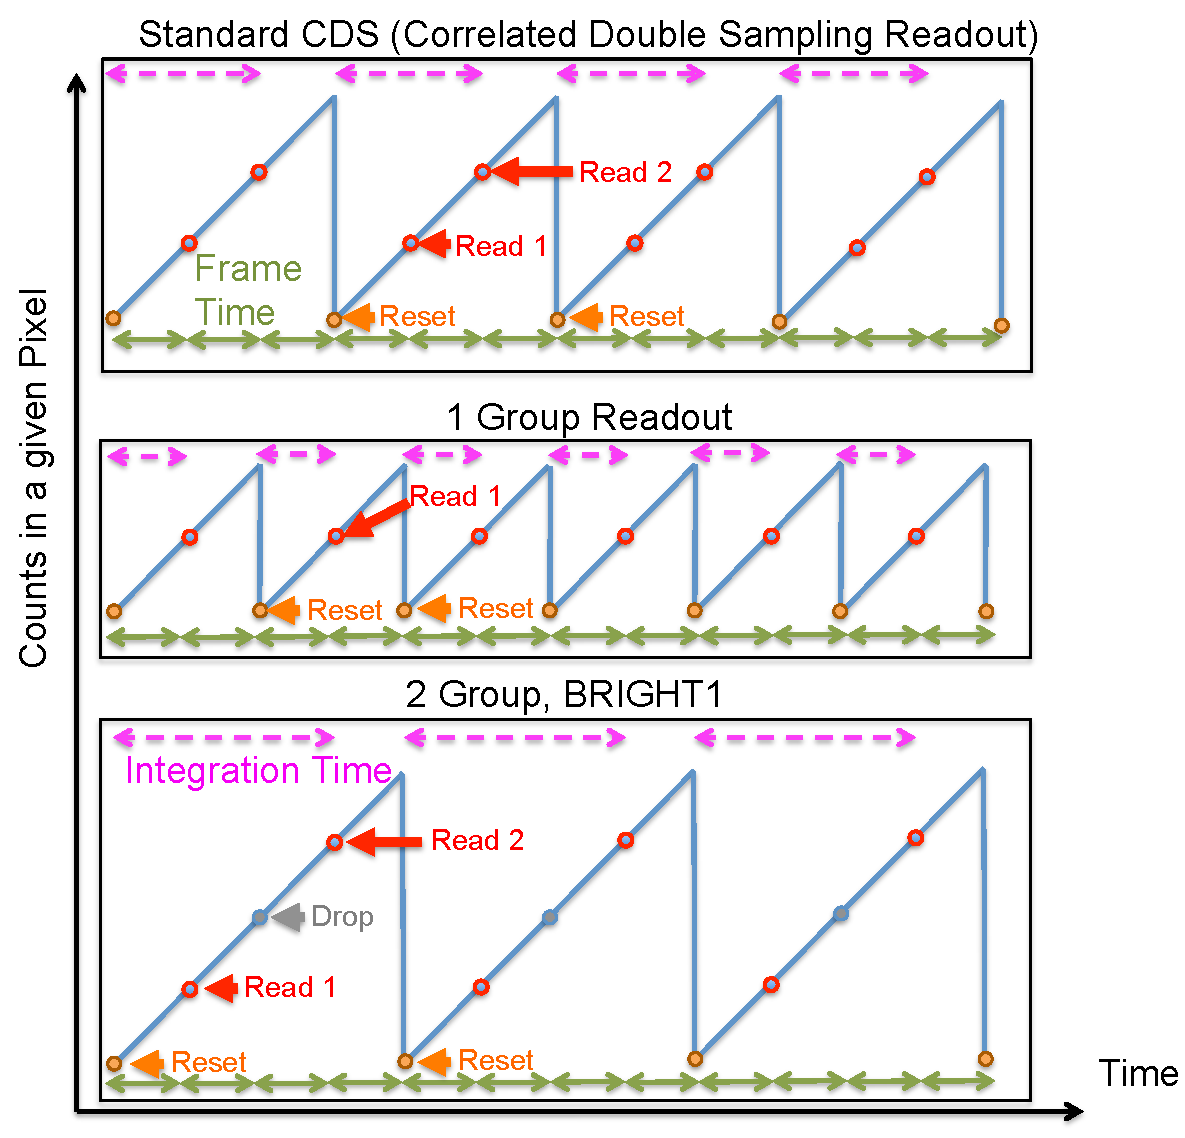
\includegraphics[width=0.5\textwidth]{readout_schematic.pdf}
\caption{Schematic of example readout modes for an exposure that is 12 frame times in duration.
A single FITS file is saved for the exposure, consisting of 1-2 groups (read 1 or both read 1 and read 2) per integration.
No reset frames or dropped frames are saved.``1 Group Readout" can be used to increase the saturation limits provided that drifts between reset levels are sufficiently stable.
The BRIGHT1 readout increases the observing efficiency and reduces data volume over CDS but will saturate more easily.}\label{fig:readout}
\end{figure}

Each NIRCam array must be read out with identical window sizes and exposure times due to restrictions in the Onboard Scripting Software (OSS).
The window sizes could theoretically be different between the long-wavelength and short-wavelength detectors with only software changes, but would require large changes to the existing software.
This means that some balance must be made between saturating the grism spectrum (which has much higher throughput) in the long-wavelength and getting the most flux in the short-wavelength DHS spectra (which have lower throughput and also spread the light over more pixels).
The current software requires that the sub-array locations must be identical for NIRCam's short wavelength arrays and long wavelength arrays.
We recommend  the sub-array locations to be adjustable so that the short wavelength sub-array can be centered on one DHS spectrum or a subset of the 10 and the long wavelength array can be centered on a single grism spectrum.
The software also is limited subarray sizes of 2048 $\times$ 64, 2048 $\times$ 128, 2048 $\times$ 256 and 2048 $\times$ 2048 (full frame), which would cover 1, 1, 2 and 10 DHS spectra.


The balance between saturating the long-wavelength grism and getting enough SNR in the DHS is listed in Table \ref{tab:SatSNRsubA}.
The table shows the brightest observable G2V star  for a given array size in the long-wavelength grism and the DHS noise at 1.5$\mu$m for a G2V type star at this brightness observing a 1 hour long transit duration and binned to a resolution of 100.
We use the standard correlated double sampling (CDS) readout mode shown in Figure \ref{fig:readout} and we consider 80\% well depth in the second read as saturation.
The sub-array sizes and order of DHS elements is shown in Figure \ref{fig:DHSaps}.
For the brightest sources, which require the 2048 $\times$ 64 pixel subarray, the DHS throughput loss is significant, because only 1 DHS spectrum out of 10 is used, meaning only about 4\% of JWST's 25 m$^2$ collecting area is used.

\begin{table}
\centering
\begin{tabular}{llll}
Sub-Array Size &  LW Saturation & \# of DHS & DHS Noise\\
                         &  K Magnitude    &                               & ppm \\
\hline \hline
2048$\times$ 64 & 4.03 & 1 &  ?? \\
2048$\times$ 200 & 5.25 & 2 &  ?? \\
2048$\times$ 500 & 6.23 & 4 &  ?? \\
2048$\times$ 1240 & 7.22 & 10 & ??
\end{tabular}
\caption{G2V-type star saturation K band limits are shown for suggested sub-array sizes.
The size affects the number of DHS that can be included, so the SNR at 1.5$\mu$m in the DHS spectrum at the given saturation limit for a 1 hour transit is shown in column 4.}\label{tab:SatSNRsubA}
\end{table}

\begin{figure}[!ht]
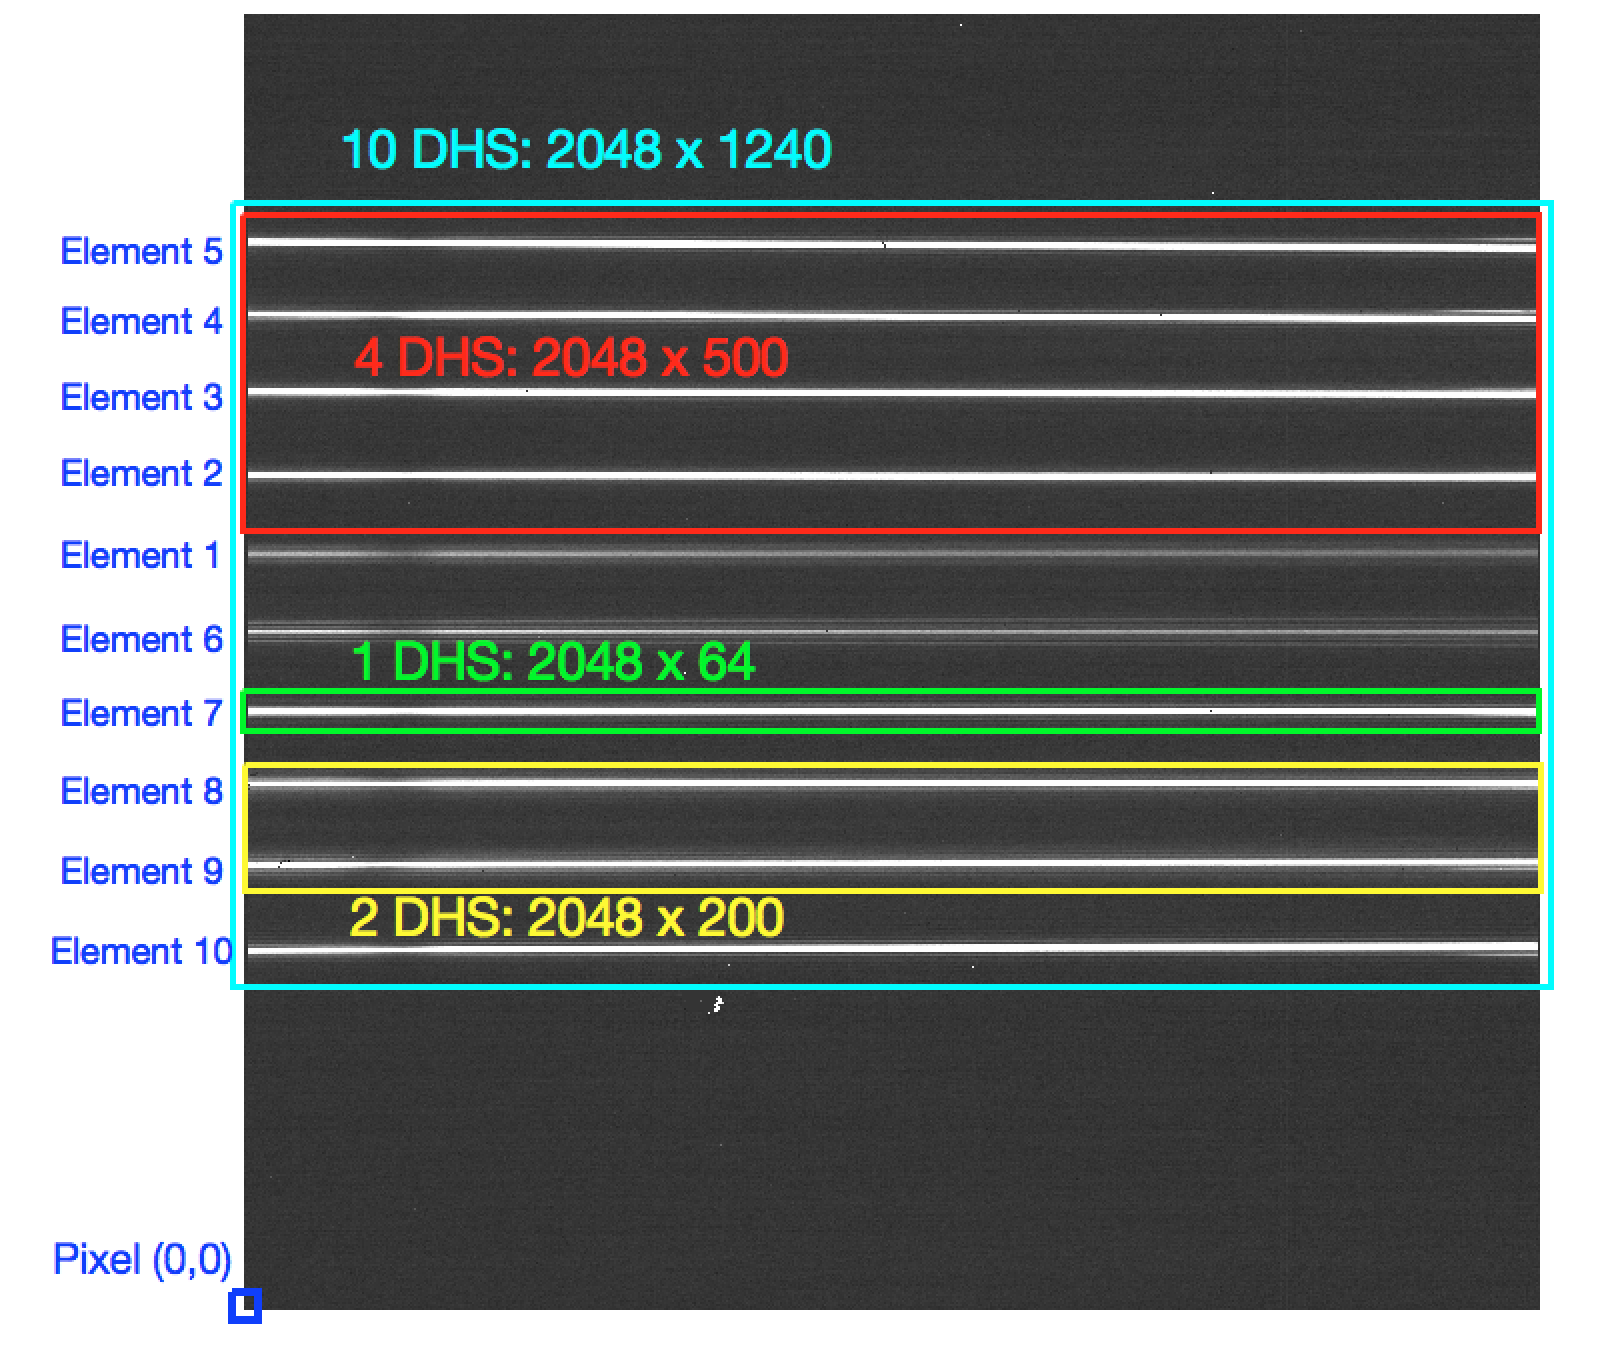
\includegraphics[width=0.5\textwidth]{example_ap_sizes.png}
\caption{Example sub-array size options for one of the short-wavelength detectors for the DHS.
Each element is labeled corresponding to the DHS apertures shown in Figure \ref{fig:DHSvsPupilOverlay}}\label{fig:DHSaps}
\end{figure}

\subsubsection{Data Volume}
For most transiting planet science, the targets are bright and so the pixels will continuously be read out and saved without any pauses or skips in the stream of data at $\sim$1.6 Mbits per second per amplifier per detector.
The amount of data streaming from the detectors can overload the Solid State Recorder (SSR), which has a capacity of 540 Gbits \citep{johns2008L2comm} (\textbf{compressed data?}).
This overload can happen in as few as 10 hours if three NIRCam detectors are used simultaneously and all are read out with four amplifiers in RAPID mode (meaning no samples are co-added or dropped).

In normal operations, up to 232 Gbits of compressed science and telemetry data from James Webb Space Telescope are downlinked once per day over the 4 hour contact time with an antenna in the Deep Space Network (SDN)  \citep{dashevsky2008groundflight}.
Science operations can continue during the 4 hour contact time, but re-pointing the high gain antenna can cause $<$0.07 \arcsec\ disturbances \citep{beichman2014pasp}.
To satisfy these normal operations, the data volume must be reduced for observations longer than \textbf{How many do you think? 6 hours to allow for telemetry and other science?} when using 3 detectors and 4 amplifiers simultaneously.

There are a few ways to reduce the data volume streaming from the detectors.
One way is to read each detector with a single amplifier (WINDOW mode).
This reduces the frame rate by a factor of four (for the four amplifiers), thus allowing $\sim$40 hours before filling JWST's solid state recorders.
The lower frame rate, however, means that the detector saturates at 1/4 the flux as four amplifiers.
Second, the detector can be read out in BRIGHT1 mode, seen in Figure \ref{fig:readout}.
This is where a frame is dropped between read 2 and read 1 to increase the integration time and efficiency while reducing data volume.
This only works for sources faint enough that the long-wavelength grisms do not saturate.
Reducing the size of the sub-array does not affect the data volume because it just increases the number of frames so that approximately the same amount of data in pixels is saved to JWST's solid state recorder.


\section{Conclusions}

The James Webb Space Telescope will provide unprecedented measurements of transiting exoplanets, especially for carbon-bearing gases in their atmospheres.
The time needed to observe in JWST's full range of wavelengths from 0.6$\mu$m to 28$\mu$m, however, can add up quickly since many transits are needed with different instrument modes to cover all wavelengths.
We introduced a new science mode using the Dispersed Hartmann Sensors on the NIRCam instrument which enable simultaneous measurements of spectra at R $\sim$ \DHSres\ from 1.0 to 2.0$\mu$m while using the NIRCam long-wavelength grisms covering either 2.4$\mu$m to 4.0$\mu$m or 3.9$\mu$m to 5.0$\mu$m.
The readout mode and subarray size must be chosen carefully on the DHS so as to not saturate the long-wavelength grisms.

The DHS mode enables more science because it has the brightest saturation limits of any JWST spectroscopic mode and can increase the wavelength coverage of a single observation.
The brightest known systems and similarly bright future TESS targets will be accessible with NIRCam's DHS mode.
We present example usage of the DHS mode on HD 209458b and show that the temperature, cloud pressure level and water vapor constraints are improved with the DHS.
Furthermore, the improved water vapor constraints also improve CO and CO$_2$ abundances because of the correlation of these derived parameters.
We encourage the implementation and approval of the DHS mode to enable this additional science in less time for this limited life observatory.

\section{Acknowledgements}

CHIMERA retrieval makes use of \texttt{emcee} \citep{foreman-mackey2013emcee} and the covariance plot was made with \texttt{corner.py} \citep{foremanCorner}.
For use of the El Gato computing system, this material is based upon work supported by the National Science Foundation under Grant No. 1228509.
Thanks to Michael Bruck at the High Performance Computing center at the University of Arizona for assisting with setting up the CHIMERA runs to utilize the HPC hardware.
%If used, some data was collected from the Open Exoplanet Catalogue \citep{rein2012openExoCat}.

%% In a manner similar to \objectname authors can provide links to dataset
%% hosted at participating data centers via the \dataset{} command.  The
%% second curly bracket argument is printed in the text while the first
%% parentheses argument serves as the valid data set identifier.  Large
%% lists of data set are best provided in a table (see Table 3 for an example).
%% Valid data set identifiers should be obtained from the data center that
%% is currently hosting the data.
%%
%% Note that AASTeX interprets everything between the curly braces in the 
%% macro as regular text, so any special characters, e.g. "#" or "_," must be 
%% preceded by a backslash. Otherwise, you will get a LaTeX error when you 
%% compile your manuscript.  Special characters do not 
%% need to be escaped in the optional, square-bracket argument.



%% In this section, we use  the \subsection command to set off
%% a subsection.  \footnote is used to insert a footnote to the text.

%% Observe the use of the LaTeX \label
%% command after the \subsection to give a symbolic KEY to the
%% subsection for cross-referencing in a \ref command.
%% You can use LaTeX's \ref and \label commands to keep track of
%% cross-references to sections, equations, tables, and figures.
%% That way, if you change the order of any elements, LaTeX will
%% automatically renumber them.

%% This section also includes several of the displayed math environments
%% mentioned in the Author Guide.


%% The equation environment wil produce a numbered display equation.


%% The \notetoeditor{TEXT} command allows the author to communicate
%% information to the copy editor.  This information will appear as a
%% footnote on the printed copy for the manuscript style file.  Nothing will
%% appear on the printed copy if the preprint or
%% preprint2 style files are used.

%% The eqnarray environment produces multi-line display math. The end of
%% each line is marked with a \\. Lines will be numbered unless the \\
%% is preceded by a \nonumber command.
%% Alignment points are marked by ampersands (&). There should be two
%% ampersands (&) per line.

%% Putting eqnarrays or equations inside the mathletters environment groups
%% the enclosed equations by letter. For instance, the eqnarray below, instead
%% of being numbered, say, (4) and (5), would be numbered (4a) and (4b).
%% LaTeX the paper and look at the output to see the results.

%% This section contains more display math examples, including unnumbered
%% equations (displaymath environment). The last paragraph includes some
%% examples of in-line math featuring a couple of the AASTeX symbol macros.

%% The displaymath environment will produce the same sort of equation as
%% the equation environment, except that the equation will not be numbered
%% by LaTeX.
%% If you wish to include an acknowledgments section in your paper,
%% separate it off from the body of the text using the \acknowledgments
%% command.

%% Included in this acknowledgments section are examples of the
%% AASTeX hypertext markup commands. Use \url without the optional [HREF]
%% argument when you want to print the url directly in the text. Otherwise,
%% use either \url or \anchor, with the HREF as the first argument and the
%% text to be printed in the second.

\acknowledgments



%% To help institutions obtain information on the effectiveness of their
%% telescopes, the AAS Journals has created a group of keywords for telescope
%% facilities. A common set of keywords will make these types of searches
%% significantly easier and more accurate. In addition, they will also be
%% useful in linking papers together which utilize the same telescopes
%% within the framework of the National Virtual Observatory.
%% See the AASTeX Web site at http://aastex.aas.org/
%% for information on obtaining the facility keywords.

%% After the acknowledgments section, use the following syntax and the
%% \facility{} macro to list the keywords of facilities used in the research
%% for the paper.  Each keyword will be checked against the master list during
%% copy editing.  Individual instruments or configurations can be provided 
%% in parentheses, after the keyword, but they will not be verified.

%{\it Facilities:} \facility{Nickel}, \facility{HST (STIS)}, \facility{CXO (ASIS)}.

%% Appendix material should be preceded with a single \appendix command.
%% There should be a \section command for each appendix. Mark appendix
%% subsections with the same markup you use in the main body of the paper.

%% Each Appendix (indicated with \section) will be lettered A, B, C, etc.
%% The equation counter will reset when it encounters the \appendix
%% command and will number appendix equations (A1), (A2), etc.

\appendix


%% The reference list follows the main body and any appendices.
%% Use LaTeX's thebibliography environment to mark up your reference list.
%% Note \begin{thebibliography} is followed by an empty set of
%% curly braces.  If you forget this, LaTeX will generate the error
%% "Perhaps a missing \item?".
%%
%% thebibliography produces citations in the text using \bibitem-\cite
%% cross-referencing. Each reference is preceded by a
%% \bibitem command that defines in curly braces the KEY that corresponds
%% to the KEY in the \cite commands (see the first section above).
%% Make sure that you provide a unique KEY for every \bibitem or else the
%% paper will not LaTeX. The square brackets should contain
%% the citation text that LaTeX will insert in
%% place of the \cite commands.

%% We have used macros to produce journal name abbreviations.
%% AASTeX provides a number of these for the more frequently-cited journals.
%% See the Author Guide for a list of them.

%% Note that the style of the \bibitem labels (in []) is slightly
%% different from previous examples.  The natbib system solves a host
%% of citation expression problems, but it is necessary to clearly
%% delimit the year from the author name used in the citation.
%% See the natbib documentation for more details and options.

\bibliographystyle{apj}
\bibliography{dhs_biblio}

%\clearpage

%% Use the figure environment and \plotone or \plottwo to include
%% figures and captions in your electronic submission.
%% To embed the sample graphics in
%% the file, uncomment the \plotone, \plottwo, and
%% \includegraphics commands
%%
%% If you need a layout that cannot be achieved with \plotone or
%% \plottwo, you can invoke the graphicx package directly with the
%% \includegraphics command or use \plotfiddle. For more information,
%% please see the tutorial on "Using Electronic Art with AASTeX" in the
%% documentation section at the AASTeX Web site, http://aastex.aas.org/
%%
%% The examples below also include sample markup for submission of
%% supplemental electronic materials. As always, be sure to check
%% the instructions to authors for the journal you are submitting to
%% for specific submissions guidelines as they vary from
%% journal to journal.

%% This example uses \plotone to include an EPS file scaled to
%% 80% of its natural size with \epsscale. Its caption
%% has been written to indicate that additional figure parts will be
%% available in the electronic journal.

%\begin{figure}
%\epsscale{.80}
%\plotone{f1.eps}
%\caption{Derived spectra for 3C138 \citep[see][]{heiles03}. Plots for all sources are available
%in the electronic edition of {\it The Astrophysical Journal}.\label{fig1}}
%\end{figure}

%\clearpage

%% Here we use \plottwo to present two versions of the same figure,
%% one in black and white for print the other in RGB color
%% for online presentation. Note that the caption indicates
%% that a color version of the figure will be available online.
%%

%\begin{figure}
%\plottwo{f2.eps}{f2_color.eps}
%\caption{A panel taken from Figure 2 of \citet{rudnick03}. 
%See the electronic edition of the Journal for a color version 
%of this figure.\label{fig2}}
%\end{figure}

%% This figure uses \includegraphics to scale and rotate the still frame
%% for an mpeg animation.

%\begin{figure}
%\includegraphics[angle=90,scale=.50]{f3.eps}
%\caption{Animation still frame taken from \citet{kim03}.
%This figure is also available as an mpeg
%animation in the electronic edition of the
%{\it Astrophysical Journal}.}
%\end{figure}

%% If you are not including electonic art with your submission, you may
%% mark up your captions using the \figcaption command. See the
%% User Guide for details.
%%
%% No more than seven \figcaption commands are allowed per page,
%% so if you have more than seven captions, insert a \clearpage
%% after every seventh one.

%% Tables should be submitted one per page, so put a \clearpage before
%% each one.

%% Two options are available to the author for producing tables:  the
%% deluxetable environment provided by the AASTeX package or the LaTeX
%% table environment.  Use of deluxetable is preferred.
%%

%% Three table samples follow, two marked up in the deluxetable environment,
%% one marked up as a LaTeX table.

%% In this first example, note that the \tabletypesize{}
%% command has been used to reduce the font size of the table.
%% We also use the \rotate command to rotate the table to
%% landscape orientation since it is very wide even at the
%% reduced font size.
%%
%% Note also that the \label command needs to be placed
%% inside the \tablecaption.

%% This table also includes a table comment indicating that the full
%% version will be available in machine-readable format in the electronic
%% edition.

%% If you use the table environment, please indicate horizontal rules using
%% \tableline, not \hline.
%% Do not put multiple tabular environments within a single table.
%% The optional \label should appear inside the \caption command.



%% If the table is more than one page long, the width of the table can vary
%% from page to page when the default \tablewidth is used, as below.  The
%% individual table widths for each page will be written to the log file; a
%% maximum tablewidth for the table can be computed from these values.
%% The \tablewidth argument can then be reset and the file reprocessed, so
%% that the table is of uniform width throughout. Try getting the widths
%% from the log file and changing the \tablewidth parameter to see how
%% adjusting this value affects table formatting.

%% The \dataset{} macro has also been applied to a few of the objects to
%% show how many observations can be tagged in a table.


%% Tables may also be prepared as separate files. See the accompanying
%% sample file table.tex for an example of an external table file.
%% To include an external file in your main document, use the \input
%% command. Uncomment the line below to include table.tex in this
%% sample file. (Note that you will need to comment out the \documentclass,
%% \begin{document}, and \end{document} commands from table.tex if you want
%% to include it in this document.)

%% \input{table}

%% The following command ends your manuscript. LaTeX will ignore any text
%% that appears after it.

\end{document}

%%
%% End of file `sample.tex'.
